%-----------------------------------------------------
\subsection{Extensions du principe d'EGO à différents contextes}
%-----------------------------------------------------
\begin{frame}
\frametitle{Extensions du principe d'EGO à différents contextes}

\begin{block}{Principe général}
\begin{itemize}
 \item Critère \textit{(statistique)} traduisant notre objectif
 \item Recherche du maximisateur du critère
 \item Ajout séquentiel de points
\end{itemize}
\end{block}

\begin{block}{Un domaine foisonnant}
\begin{itemize}
 \item Parallélisation
 \item Modèles stochastiques, optimisation avec paramètres incertains
 \item Optimisation sous contraintes, multi-objectif, multi-fidélité
  \item Alternatives à l'EI
 \item Autres modèles : par ex. Bayesian additive regression trees
 \scriptsize{
 \begin{thebibliography}{7}
\beamertemplatearticlebibitems
%\beamertemplatebookbibitems
     \bibitem{chi}
    Chipman et al. (2009)
         \newblock Sequential Design for Computer Experiments with a Flexible Bayesian Additive Model
 \end{thebibliography}}
\end{itemize}
\end{block}
\end{frame}

%-----------------------------------------------------
\begin{frame}
\frametitle{Parallélisation}

\begin{block}{Ajout de plusieurs points simultanément au lieu d'un seul}
L'amélioration est apportée par le meilleur des points :
$$EI(x_1, \ldots, x_p) = \mathbb{E} \left[ \left(y_{min} - \min(Y(x_1), \ldots, Y(x_p) \right)^+   \right]$$
\end{block}

\scriptsize{
 \begin{thebibliography}{7}
\beamertemplatearticlebibitems
%\beamertemplatebookbibitems
     \bibitem{bay}
     M.~Taddy, H.~Lee, G.~Gray, J.~Griffin (2009)
         \newblock Bayesian guided pattern search for robust local optimization
         \newblock Technometrics, 51(4), 389-401

     \bibitem{para}
     D.~Ginsbourger, R.~Le Riche, L.~Carraro (2010)
         \newblock Kriging is well-suited to parallelize optimization
         \newblock Computational intelligence in expensive optimization problems, 131-162 
 \end{thebibliography}
}
\end{frame}

%-----------------------------------------------------
\begin{frame}
\frametitle{Multi-objectifs : un métamodèle par objectif}
 ``Amélioration'' sur le front de Pareto ?

\scriptsize{
 \begin{thebibliography}{2}
\beamertemplatearticlebibitems
\bibitem{para}
     J.~Svenson (2011)
         \newblock Computer experiments: multiobjective optimization and sensitivity analysis, \textcolor{blue}{PhD thesis, Ohio State University}
         \bibitem{moi}
     V.~Picheny (2014)
         \newblock Multiobjective optimization using Gaussian process emulators via stepwise uncertainty reduction, \textcolor{blue}{Statistics and Computing}
\end{thebibliography}
}
\begin{figure}[h!]
  \centering
  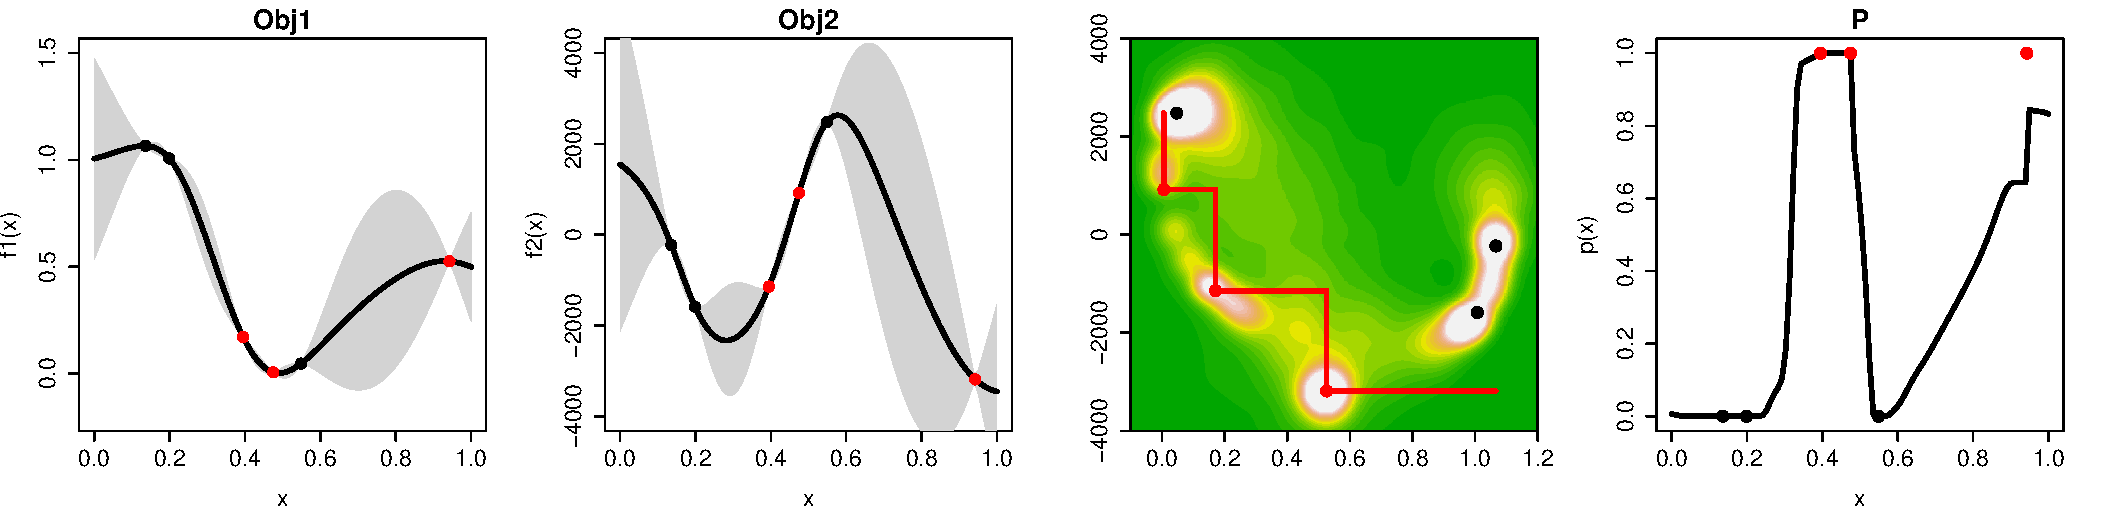
\includegraphics[trim=0 0 90mm 0, width=.9\paperwidth, clip]{fig/multiPGinitFull.pdf}
\end{figure}

\normalsize
\texttt{R} package \textcolor{blue}{\texttt{GPareto}}
\end{frame}
%-----------------------------------------------------
\begin{frame}
\frametitle{Optimisation avec contraintes : 3 cas (1/2)}
\begin{columns}[t]
 \begin{column}{.49\textwidth}
  \begin{block}{Objectif coûteux, contrainte rapide}
$$\begin{array}{ll}
 \max & \text{Rendement}\\
 s.c. & \text{ITK réalisable}
\end{array}$$
\vspace{-3mm}
\begin{itemize}
 \item Métamodèle pour l'objectif
 \item EGO classique avec contrainte sur la maximisation de l'EI
\end{itemize}
\end{block}
\vspace{1cm}
\scriptsize{
 \begin{thebibliography}{7}
\beamertemplatearticlebibitems
\bibitem{kriginv}
     Chevalier, Picheny, Ginsbourger (2014)
         \newblock KrigInv: An efficient and user-friendly implementation of batch-sequential inversion strategies based on kriging,
         \newblock  CSDA, vol.71, pp.1021-1034
\end{thebibliography}}
 \end{column}
 
\begin{column}{.49\textwidth}
 \begin{block}{Objectif rapide, contrainte coûteuse}
 \vspace{-4mm}
$$\begin{array}{ll}
 \min & \text{Poids}\\
 s.c. & \text{Contrainte méca.} \leq \text{Seuil}
\end{array}$$
\vspace{-4mm}
\begin{itemize}
 \item Métamodèle pour la contrainte
 \item Apprentissage de la frontière
\end{itemize}
\end{block}
\centering
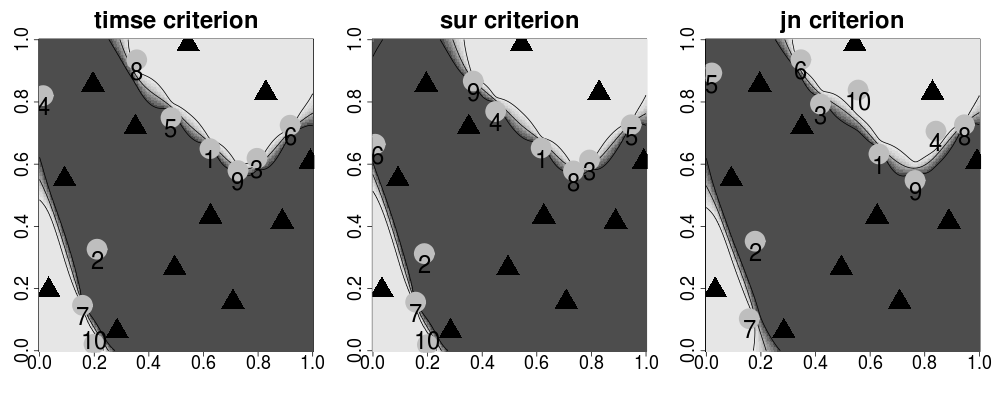
\includegraphics[trim= 235mm 0mm 0mm 0mm, clip, width=.53\textwidth]{fig/integralcriteria.png}
\end{column}
\end{columns}
\end{frame}
%-----------------------------------------------------
\begin{frame}
\frametitle{Optimisation avec contraintes : 3 cas (2/2)}

\begin{block}{Objectif \& contraintes coûteux \textit{(ou : contrainte de crash)}}
\begin{itemize}
 \item Un métamodèle pour chaque fonction
 \item ``Amélioration faisable'' ?
\end{itemize}
\end{block}

\begin{figure}[h!]
  \centering	
  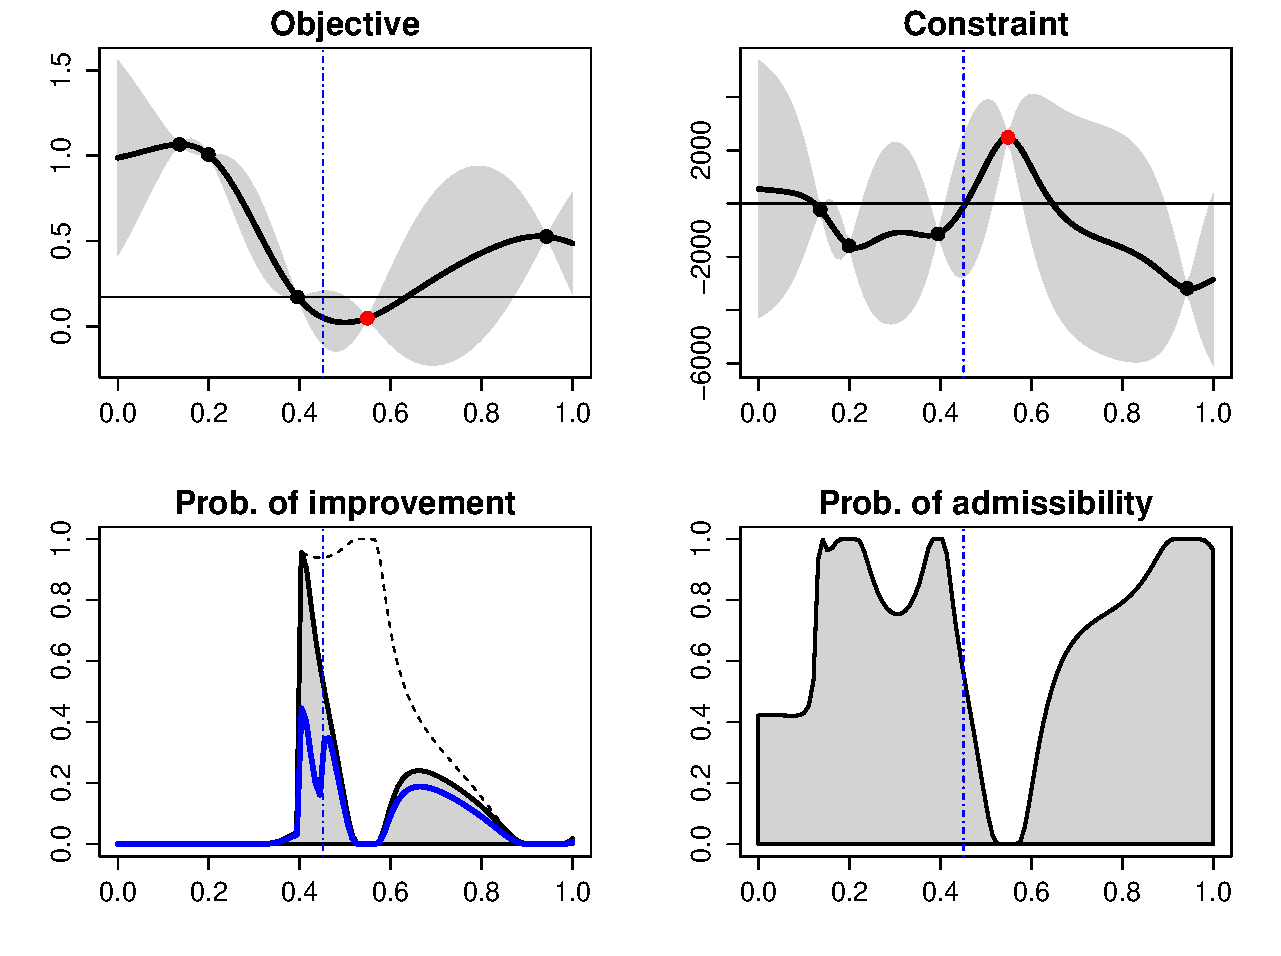
\includegraphics[trim= 0mm 0mm 0mm 0mm, clip, width=.56\textwidth]{fig/cst1Dillus.pdf}
\end{figure}
\end{frame}
%-----------------------------------------------------
\begin{frame}
\frametitle{Alternatives à l'EI : critères spatialisés}

\begin{columns}[t]
\begin{column}{6cm}
\begin{block}{IAGO : Informal Approach to Global Optimization}
Réduction de l'entropie du minimum
\end{block}

\begin{block}{IECI : Integrated Expected Conditional Improvement}
Gain estimé sur tout l'espace
\end{block}

\begin{block}{EEV : Expected Volume Reduction}
Réduction du volume sous le minimum
\end{block}

\end{column}

\begin{column}{6cm}
Distribution du minimum (IAGO) :
\begin{figure}
	\centering
		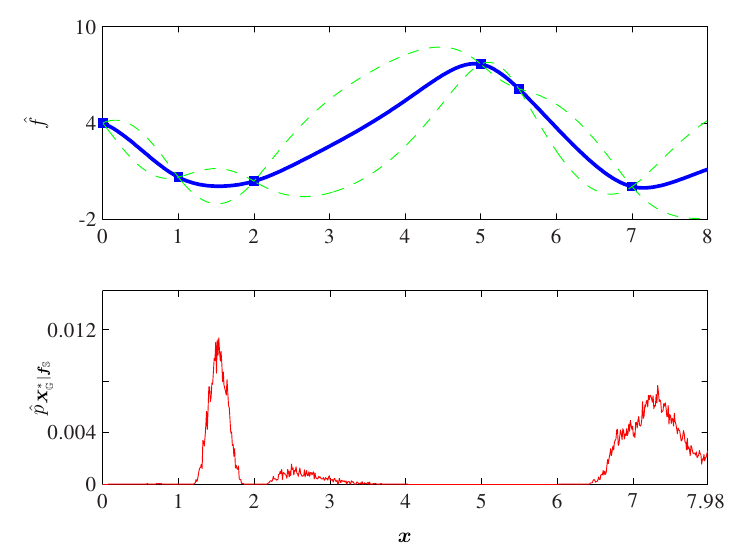
\includegraphics[width=50mm]{fig/iago.png}
\end{figure}

\scriptsize{
 \begin{thebibliography}{1}
\beamertemplatearticlebibitems
%\beamertemplatebookbibitems
     \bibitem{iago}
     J.~Villemonteix, E.~Vazquez, E.~Walter (2009)
         \newblock An informational approach to the global optimization of expensive-to-evaluate functions
         \newblock Journal of Global Optimization       
 \end{thebibliography}
}
\end{column}
\end{columns}
\end{frame}
%-----------------------------------------------------
\begin{frame}
\frametitle{Modèles complexes (1/2) : krigeages non stationnaires}
\vspace{-8mm}
\begin{columns}[t]
 \begin{column}{.49\textwidth}
 \begin{block}{Déformation de l'espace : \textit{scaling}} 
 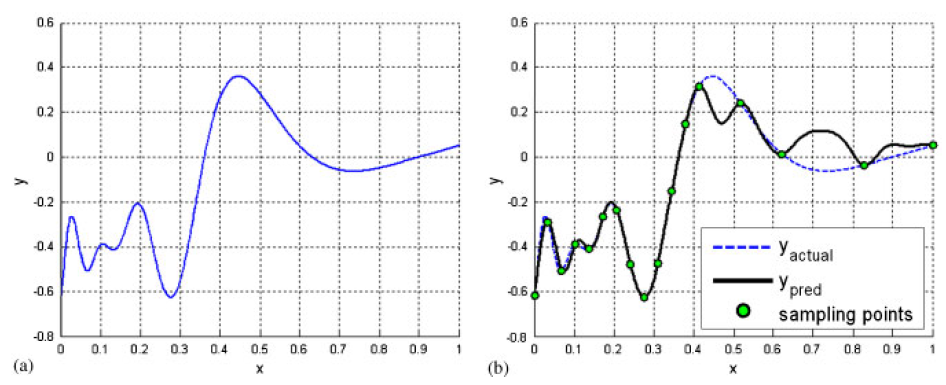
\includegraphics[trim= 0mm 0mm 0mm 0mm, clip, width=\textwidth]{fig/nonSTkrig1.png}
 
 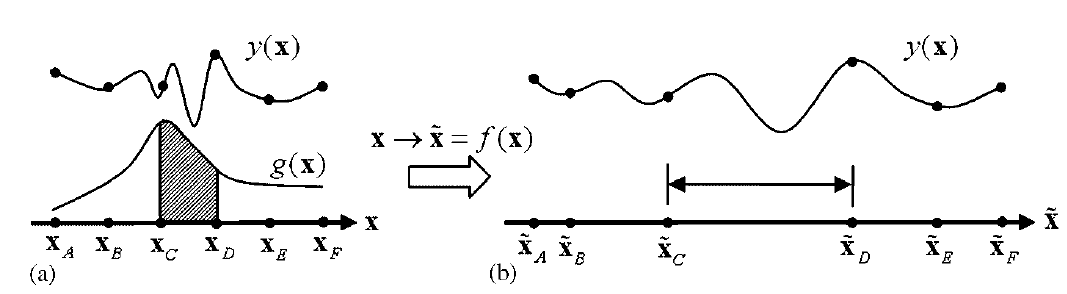
\includegraphics[trim= 0mm 0mm 0mm 0mm, clip, width=\textwidth]{fig/nonSTkrig2.png}

 \scriptsize{
 \begin{thebibliography}{1}
\beamertemplatearticlebibitems
%\beamertemplatebookbibitems
     \bibitem{nonst}
 Xiong, Chen, Apley, Ding (2007)
\newblock A non-stationary covariance-based Kriging method for metamodelling in engineering design
\newblock Int. J. for Num. Meth. in Eng.
\end{thebibliography}
}
% \textcolor{red}{Déformation satisfaisante avec peu de paramètres ?}
 \end{block}
 \end{column}
 \begin{column}{.49\textwidth}
  \begin{block}{Découpage de l'espace : treed GP}
\centering
   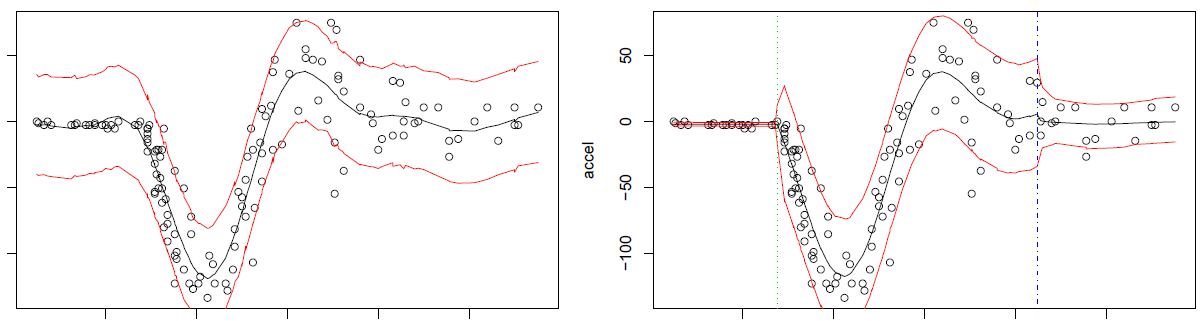
\includegraphics[trim= 0mm 0mm 225mm 0mm, clip, width=.85\textwidth]{fig/tgp.png}
 
 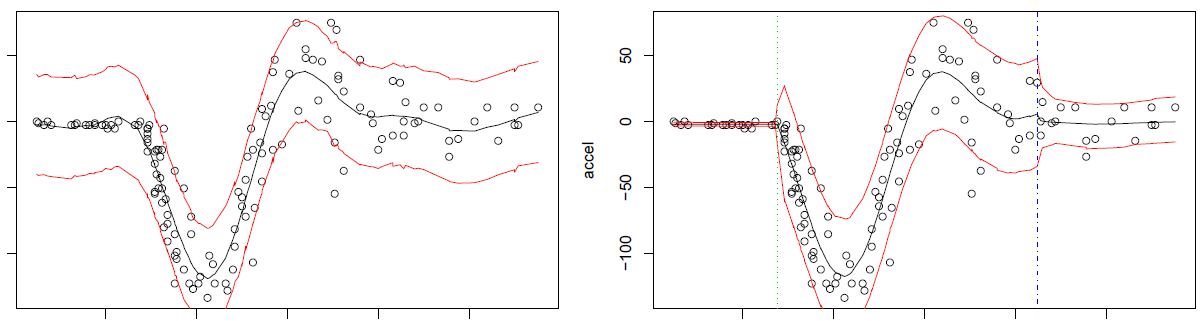
\includegraphics[trim= 225mm 0mm 0mm 0mm, clip, width=.85\textwidth]{fig/tgp.png}
  
\end{block}
 \end{column}
\end{columns}

\vspace{5mm}
\textcolor{red}{$\qquad \qquad \Rightarrow$ EGO directement applicable}
\end{frame}

%-----------------------------------------------------
\begin{frame}
\frametitle{Modèles complexes (2/2) : ajout d'informations}

\begin{block}{Les processus gaussiens peuvent inclure beaucoup d'information !}
\begin{figure}
	\centering
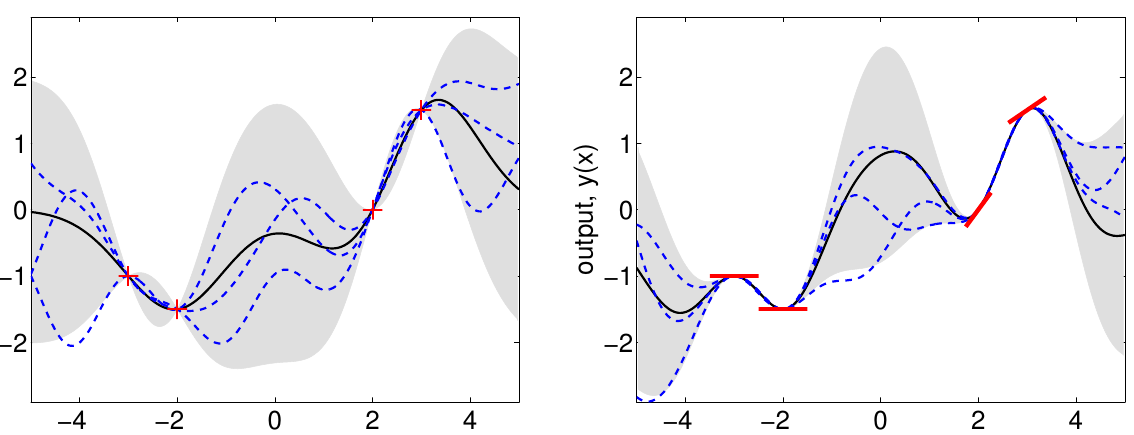
\includegraphics[trim= 0mm 0mm 0mm 0mm, clip, width=.8\textwidth]{fig/derivativeGP.png}
 \end{figure}
 \scriptsize  \textit{source : Gaussian Process for Machine Learning (2006)}
\end{block}
\normalsize
\begin{block}{Mais également conditions au bord, symétries...}
Presque tout est envisageable si on trouve la distance / covariance adaptée
\end{block}
\end{frame}

%-----------------------------------------------------
\begin{frame}
\frametitle{Pour finir : de nombreux sujets non abordés...}
\begin{block}{...par manque de temps !}
\begin{itemize}
 \item Optimisation robuste (ou fiabiliste)
 \item Optimisation bruitée
 \item Multi-fidélité
 \item Grande dimension
 \item ...
\end{itemize}
\end{block}
\end{frame}